Para analizar la calidad del algoritmo realizamos dos tipos diferentes de benchmark, uno que cuantifica la dispersión
media de distintas ejecuciones con distintas semillas para cada algoritmo y otro que estima después de un número
determinado de ejecuciones el tiempo de ejecución medio de cada algoritmo para cada dataset. Cuanto más se aproxime
a cero la dispersión mejor será el algoritmo. A iguales dispersiones consideraremos que un algoritmo es mejor que otro
si el tiempo de ejecución es significativamente menor.

Para el caso de los algoritmos genéticos, a diferencia de para los casos de los algoritmos Greedy y BL, recogeremos 
por cada fichero de benchmark la solución que nos proporcione el algoritmo en cuestión, para una única semilla. Procedemos
de igual forma para el caso de los algoritmos meméticos.

\begin{minipage}{\textwidth}
    \section{Procedimiento para la obtención de resultados}
    
    Los resultados disponibles en los cuadros de esta sección han sido resultado de distintas ejecuciones.
    
    Para obtener la dispersión hemos ejecutado el algoritmo para cada dataset para 5 semillas distintas disponibles
    en el script lanzador. Cada fila de los cuadros 3 y 4 corresponde a la dispersión media de los 5 resultados de cada
    una de estas ejecuciones (para los algoritmos que corresponda)
    
    Por otra parte, para obtener el tiempo medio de ejecución para fila de las tablas hemos ejecutado cada dataset
    para 5 semillas unas 50 veces en invocaciones diferentes y obtenido la media de los resultados del tiempo de estas
    $ 50 \cdot 5 $ ejecuciones (para los algoritmos que corresponda)
    
    Por último hemos calculado la desviación media de las soluciones para cada tabla como la suma de las desviaciones
    entre el número de casos, símil para el caso del cálculo del tiempo medio. La desviación la hemos calculado como la
    diferencia entre el coste en dispersión de nuestro algoritmo y el coste de nuestra referencia.
    
\end{minipage}

\begin{table}[!ht]%
    \centering
    \begin{tabular}{|l|l|l|}
        \hline
        \textbf{Algoritmo} & \textbf{Desviación~Media} & \textbf{Tiempo~(s)} \\ \hline
        Greedy & 129,45 & 1,53E-03 \\ \hline
        Búsqueda~Local~Primer~Mejor & 87,28 & 1,57E-02 \\ \hline
        Búsqueda~Local & 97,79 & 1,56E-02 \\ \hline
        AGG-uniforme & 77,38 & 5,38E+00 \\ \hline
        AGG-posicion & 92,22 & 1,10E+00 \\ \hline
        AGE-uniforme & 29,88 & 8,81E+00 \\ \hline
        AGE-posicion & 42,15 & 9,54E-01 \\ \hline
        Memetico-10-1.0 & 22,72 & 3,69E+01 \\ \hline
        Memetico-10-0.1 & 42,99 & 3,00E+01 \\ \hline
        Memetico-10-0.1best & 32,94 & 2,97E+01 \\ \hline
    \end{tabular}
\caption{Tabla resumen de las ejecuciones. A menor dispersión mejor resultado.}
\end{table}

\section{Análisis de los datos obtenidos}

Una vez extraidos los datos observamos cómo los algoritmos que implementamos nos ofrecen
soluciones sustancialmente diferentes según las semillas que empleamos, especialmente en
aquellos en los que parten de una única solución generada aleatoriamente. Parece que existe
cierta correlación entre una exploración más amplia del espacio de soluciones y
la obtención de mejores resultados.

\begin{figure}[H]
    \centering
    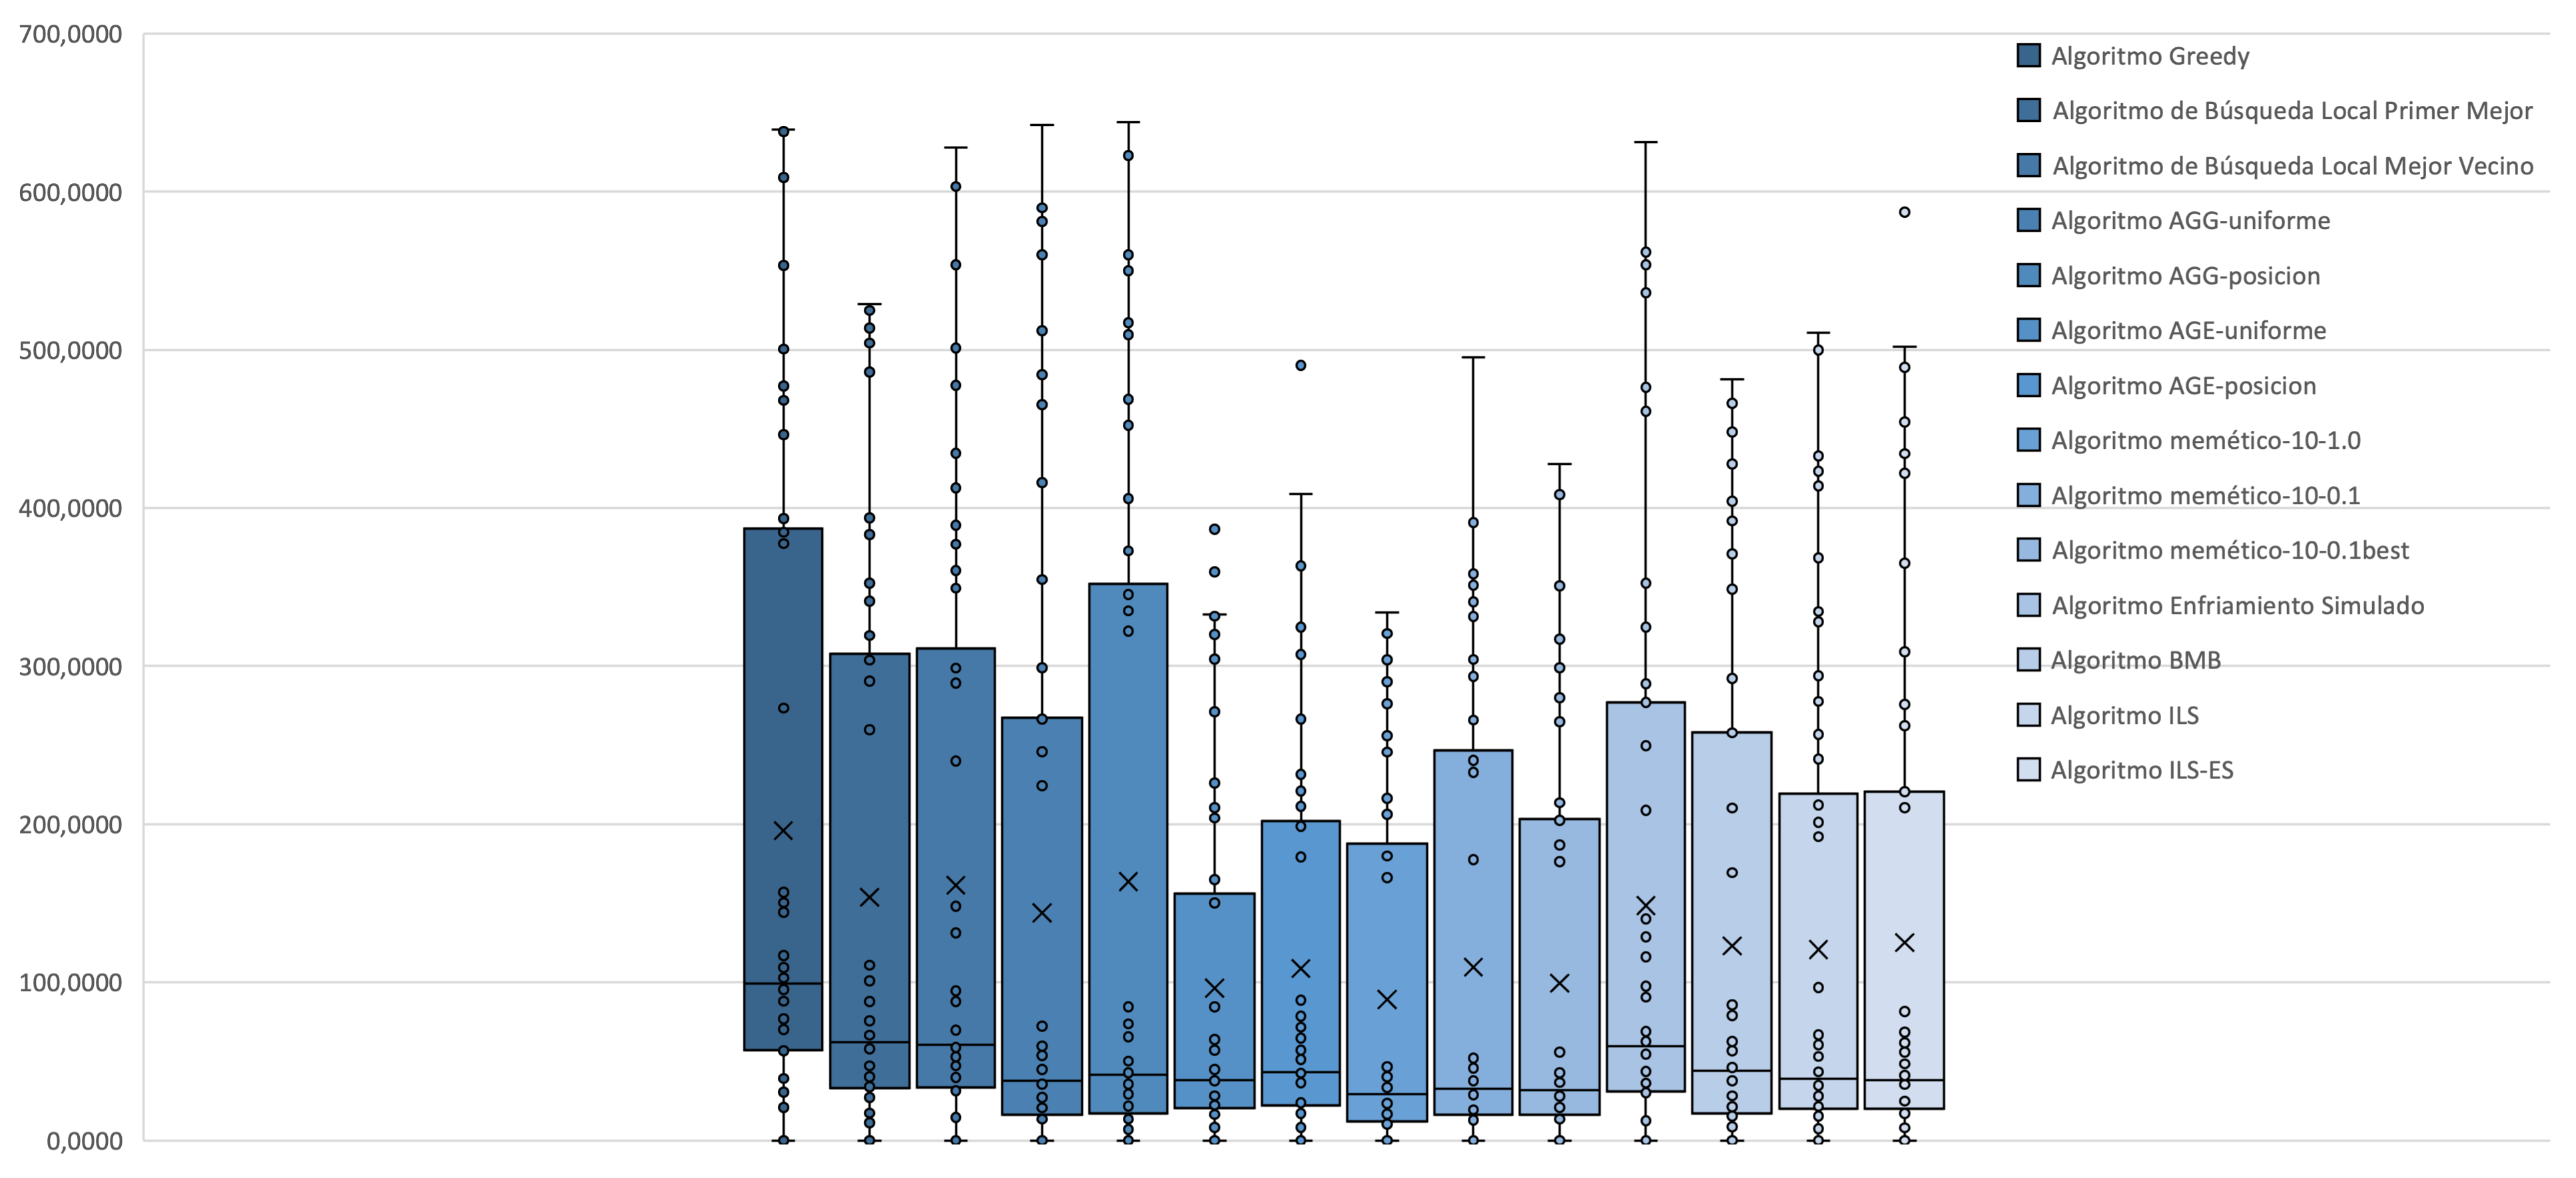
\includegraphics[keepaspectratio,width=\textwidth]{box_and_whisker_dispersion_media_dataset_y_tipo_algoritmo.png}
    \caption{Dispersión media por dataset y por tipo de algoritmo. Podemos observar que hay una alta desviación típica del coste de las soluciones.
    Podemos ver que una peor media de resultados en las ejecuciones no implica una peor mediana, y una peor mediana no implica un intervalo del percentil 25 al 75 peor.
    Destacamos también la correlación entre medianas dentro de un mismo tipo de algoritmo.}
\end{figure}

Para aumentar el espacio en el espacio de soluciones del conjunto de soluciones consideradas por los algoritmos Greedy y de Búsqueda Local y no quedar
así atrapados en óptimos locales utilizando estrategias de BL podríamos probar variantes como la Búsqueda Local Estocástica, Búsqueda Local por Primer Mejor Aleatorio, Búsqueda Local
con Reinicio Aleatorio u otras técnicas más avanzadas como el Enfriamiento Simulado o búsqueda \textit{Local Beam} entre otros.\cite[Sección 4.1]{russell2020artificial}

Probamos con las técnicas Búsqueda Local con Reinicio Aleatorio y Búsqueda Reiterada por BL y ES.
Podemos observar cómo, aun teniendo como base una búsqueda local, las soluciones obtenidas son significativamente mejores, observando de nuevo como destacábamos anteriormente
correlación entre una mayor exploración del espacio de soluciones y mejores soluciones.
Sin embargo esto no ocurre así para las ejecuciones del algoritmo de Enfriamiento Simulado. Podemos ver que ofrece soluciones un tanto mejores que una búsqueda local, pero bastante
peores que estos. Haciendo pruebas vemos cómo la función de aceptación probabilística
es significativamente determinante en los resultados finales obtenidos. Sospechamos que el no ofrecer mejores soluciones
es causa del operador de mutación del algoritmo, que no produce soluciones suficientemente diversas. Sin embargo no tenemos certeza en la causalidad,
sólo en los resultados obtenidos.

Otra opción para aumentar el espacio es la de usar algoritmos genéticos. Podemos ver que ofrecen unos muy buenos resultados, gracias a que no sólo van saltando más por el espacio de soluciones
sino que además van conservando las partes de las soluciones más prometedoras, alejándolos de una simple búsqueda aleatoria. Podemos ver cómo para el problema del MDD los modelos
estacionarios dan mejores soluciones que los generacionales. Esto se puede deber a que los generacionales sustituyen completamente la población original, mientras que los estacionarios
únicamente inserta las nuevas soluciones en la población inicial si estas son mejores, conservando más información acerca de las soluciones más prometedoras y no cayendo tanto en la aleatoriedad.

De igual forma podemos destacar cómo el operador de cruce uniforme ofrece mejores resultados que el de posición. Esto se debe a que ambos cruces, aunque mantienen la intersección de genes,
aleatorizan los genes que quedan por escoger. Sin embargo el cruce uniforme, al reparar la solución, va buscando y eliminando los genes que más le convenga, aplicando un esquema Greedy, que
seguramente ayudará a obtener soluciones con mejor fitness.

En nuestras ejecuciones los algoritmos meméticos, aunque mejores que una búsqueda local, dan peor rendimiento que el resto de algoritmos genéticos.
En este, cuanto más peso le damos al paso genético y cuanto más fuerte sea el elitismo, da mejores resultados.

\subsection{Conclusiones}

En el problema del MDD, para nuestras implementaciones de los algoritmos de búsqueda por trayectorias y de búsqueda por
poblaciones, comprobamos que los más efectivos son los genéticos AGE, meméticos, búsquedas reiteradas y búsquedas con
reinicio aleatorio. Es decir, existe una correlación entre aquellos que combinan una exploración del espacio de soluciones
más o menos amplio pero optimizando las soluciones por medio de búsquedas locales o parecidos y un mejor resultado en las
soluciones que obtenemos. Obtenemos mejores medias que otros métodos, como el acercamiento greedy, búsquedas locales y genéticos AGG.

\pagebreak

\begin{table}[!ht]%
    \centering    
    \begin{adjustbox}{height=12cm}
    \begin{tabular}{|l|l|l|l|}
    \hline
        Caso & Coste~Medio~Obtenido & Desv & Tiempo~(s) \\ \hline
        GKD-b\_1\_n25\_m2 & 0,0000 & 0,00 & 1,22E-05 \\ \hline
        GKD-b\_2\_n25\_m2 & 0,0000 & 0,00 & 1,36E-05 \\ \hline
        GKD-b\_3\_n25\_m2 & 0,0000 & 0,00 & 1,31E-05 \\ \hline
        GKD-b\_4\_n25\_m2 & 0,0000 & 0,00 & 1,17E-05 \\ \hline
        GKD-b\_5\_n25\_m2 & 0,0000 & 0,00 & 1,14E-05 \\ \hline
        GKD-b\_6\_n25\_m7 & 70,9064 & 58,19 & 5,11E-05 \\ \hline
        GKD-b\_7\_n25\_m7 & 57,0336 & 42,93 & 4,77E-05 \\ \hline
        GKD-b\_8\_n25\_m7 & 44,6512 & 27,89 & 5,08E-05 \\ \hline
        GKD-b\_9\_n25\_m7 & 57,4252 & 40,36 & 5,40E-05 \\ \hline
        GKD-b\_10\_n25\_m7 & 73,3526 & 50,09 & 5,98E-05 \\ \hline
        GKD-b\_11\_n50\_m5 & 20,9113 & 18,99 & 6,85E-05 \\ \hline
        GKD-b\_12\_n50\_m5 & 25,0564 & 22,94 & 7,73E-05 \\ \hline
        GKD-b\_13\_n50\_m5 & 24,8575 & 22,50 & 8,35E-05 \\ \hline
        GKD-b\_14\_n50\_m5 & 30,4310 & 28,77 & 8,29E-05 \\ \hline
        GKD-b\_15\_n50\_m5 & 39,1907 & 36,34 & 8,00E-05 \\ \hline
        GKD-b\_16\_n50\_m15 & 158,8222 & 116,08 & 4,10E-04 \\ \hline
        GKD-b\_17\_n50\_m15 & 150,3960 & 102,29 & 4,11E-04 \\ \hline
        GKD-b\_18\_n50\_m15 & 156,8830 & 113,69 & 4,32E-04 \\ \hline
        GKD-b\_19\_n50\_m15 & 151,8338 & 105,42 & 3,96E-04 \\ \hline
        GKD-b\_20\_n50\_m15 & 145,6224 & 97,91 & 3,48E-04 \\ \hline
        GKD-b\_21\_n100\_m10 & 78,0183 & 64,19 & 3,79E-04 \\ \hline
        GKD-b\_22\_n100\_m10 & 76,9076 & 63,24 & 3,50E-04 \\ \hline
        GKD-b\_23\_n100\_m10 & 81,3711 & 66,03 & 3,44E-04 \\ \hline
        GKD-b\_24\_n100\_m10 & 79,6570 & 71,02 & 3,68E-04 \\ \hline
        GKD-b\_25\_n100\_m10 & 56,6460 & 39,45 & 3,43E-04 \\ \hline
        GKD-b\_26\_n100\_m30 & 377,4836 & 208,75 & 1,98E-03 \\ \hline
        GKD-b\_27\_n100\_m30 & 446,3368 & 319,24 & 2,08E-03 \\ \hline
        GKD-b\_28\_n100\_m30 & 384,7054 & 278,33 & 2,01E-03 \\ \hline
        GKD-b\_29\_n100\_m30 & 273,4050 & 135,95 & 1,98E-03 \\ \hline
        GKD-b\_30\_n100\_m30 & 393,1588 & 265,68 & 2,08E-03 \\ \hline
        GKD-b\_31\_n125\_m12 & 70,1099 & 58,36 & 5,46E-04 \\ \hline
        GKD-b\_32\_n125\_m12 & 89,5372 & 70,75 & 5,56E-04 \\ \hline
        GKD-b\_33\_n125\_m12 & 88,0445 & 69,51 & 5,52E-04 \\ \hline
        GKD-b\_34\_n125\_m12 & 73,3446 & 53,86 & 6,36E-04 \\ \hline
        GKD-b\_35\_n125\_m12 & 95,3074 & 77,19 & 6,45E-04 \\ \hline
        GKD-b\_36\_n125\_m37 & 468,0492 & 312,61 & 3,97E-03 \\ \hline
        GKD-b\_37\_n125\_m37 & 500,5334 & 301,64 & 4,27E-03 \\ \hline
        GKD-b\_38\_n125\_m37 & 553,3864 & 365,42 & 4,17E-03 \\ \hline
        GKD-b\_39\_n125\_m37 & 479,3044 & 310,71 & 4,37E-03 \\ \hline
        GKD-b\_40\_n125\_m37 & 501,5562 & 323,36 & 4,25E-03 \\ \hline
        GKD-b\_41\_n150\_m15 & 113,3785 & 90,03 & 1,14E-03 \\ \hline
        GKD-b\_42\_n150\_m15 & 144,4201 & 117,63 & 1,09E-03 \\ \hline
        GKD-b\_43\_n150\_m15 & 116,8756 & 90,12 & 1,05E-03 \\ \hline
        GKD-b\_44\_n150\_m15 & 109,1999 & 83,26 & 1,04E-03 \\ \hline
        GKD-b\_45\_n150\_m15 & 102,7905 & 75,02 & 1,01E-03 \\ \hline
        GKD-b\_46\_n150\_m45 & 637,9208 & 410,17 & 6,46E-03 \\ \hline
        GKD-b\_47\_n150\_m45 & 477,0816 & 248,48 & 6,39E-03 \\ \hline
        GKD-b\_48\_n150\_m45 & 609,1548 & 382,41 & 6,57E-03 \\ \hline
        GKD-b\_49\_n150\_m45 & 639,2372 & 412,83 & 6,60E-03 \\ \hline
        GKD-b\_50\_n150\_m45 & 471,5032 & 222,65 & 6,38E-03 \\ \hline
    \end{tabular}
    \end{adjustbox}
    \caption{Resultados de la ejecución del algoritmo \textbf{Greedy}}
\end{table}

\pagebreak
\pagebreak

\begin{table}[!ht]
    \centering
    \begin{adjustbox}{height=12cm}
    \begin{tabular}{|l|l|l|l|}
    \hline
        Caso & Coste medio obtenido & Desv & Tiempo~(s) \\ \hline
        GKD-b\_1\_n25\_m2 & 0,0000 & 0,00 & 1,86E-05 \\ \hline
        GKD-b\_2\_n25\_m2 & 0,0000 & 0,00 & 1,70E-05 \\ \hline
        GKD-b\_3\_n25\_m2 & 0,0000 & 0,00 & 1,89E-05 \\ \hline
        GKD-b\_4\_n25\_m2 & 0,0000 & 0,00 & 1,76E-05 \\ \hline
        GKD-b\_5\_n25\_m2 & 0,0000 & 0,00 & 1,72E-05 \\ \hline
        GKD-b\_6\_n25\_m7 & 30,5731 & 17,86 & 2,73E-04 \\ \hline
        GKD-b\_7\_n25\_m7 & 27,2974 & 13,20 & 2,16E-04 \\ \hline
        GKD-b\_8\_n25\_m7 & 42,2687 & 25,51 & 2,41E-04 \\ \hline
        GKD-b\_9\_n25\_m7 & 40,2675 & 23,20 & 2,42E-04 \\ \hline
        GKD-b\_10\_n25\_m7 & 45,7940 & 22,53 & 2,23E-04 \\ \hline
        GKD-b\_11\_n50\_m5 & 15,5196 & 13,59 & 2,80E-04 \\ \hline
        GKD-b\_12\_n50\_m5 & 11,3000 & 9,18 & 2,35E-04 \\ \hline
        GKD-b\_13\_n50\_m5 & 13,1555 & 10,79 & 2,84E-04 \\ \hline
        GKD-b\_14\_n50\_m5 & 21,0886 & 19,43 & 2,26E-04 \\ \hline
        GKD-b\_15\_n50\_m5 & 17,2445 & 14,39 & 2,65E-04 \\ \hline
        GKD-b\_16\_n50\_m15 & 100,7846 & 58,04 & 2,99E-03 \\ \hline
        GKD-b\_17\_n50\_m15 & 115,8601 & 67,75 & 3,04E-03 \\ \hline
        GKD-b\_18\_n50\_m15 & 87,7141 & 44,52 & 2,18E-03 \\ \hline
        GKD-b\_19\_n50\_m15 & 110,8314 & 64,42 & 2,26E-03 \\ \hline
        GKD-b\_20\_n50\_m15 & 112,7244 & 65,01 & 2,84E-03 \\ \hline
        GKD-b\_21\_n100\_m10 & 33,8073 & 19,98 & 2,09E-03 \\ \hline
        GKD-b\_22\_n100\_m10 & 47,3694 & 33,71 & 1,76E-03 \\ \hline
        GKD-b\_23\_n100\_m10 & 38,7309 & 23,39 & 1,94E-03 \\ \hline
        GKD-b\_24\_n100\_m10 & 37,8747 & 29,23 & 2,02E-03 \\ \hline
        GKD-b\_25\_n100\_m10 & 36,5649 & 19,36 & 1,96E-03 \\ \hline
        GKD-b\_26\_n100\_m30 & 383,0796 & 214,35 & 1,40E-02 \\ \hline
        GKD-b\_27\_n100\_m30 & 319,3224 & 192,23 & 2,10E-02 \\ \hline
        GKD-b\_28\_n100\_m30 & 259,7818 & 153,40 & 2,38E-02 \\ \hline
        GKD-b\_29\_n100\_m30 & 290,5872 & 153,13 & 2,09E-02 \\ \hline
        GKD-b\_30\_n100\_m30 & 303,7936 & 176,31 & 1,95E-02 \\ \hline
        GKD-b\_31\_n125\_m12 & 48,1569 & 36,41 & 3,34E-03 \\ \hline
        GKD-b\_32\_n125\_m12 & 47,2372 & 28,45 & 3,30E-03 \\ \hline
        GKD-b\_33\_n125\_m12 & 43,2685 & 24,74 & 3,68E-03 \\ \hline
        GKD-b\_34\_n125\_m12 & 48,4522 & 28,96 & 3,77E-03 \\ \hline
        GKD-b\_35\_n125\_m12 & 57,8748 & 39,76 & 3,19E-03 \\ \hline
        GKD-b\_36\_n125\_m37 & 341,0166 & 185,58 & 4,36E-02 \\ \hline
        GKD-b\_37\_n125\_m37 & 524,9386 & 326,04 & 4,93E-02 \\ \hline
        GKD-b\_38\_n125\_m37 & 514,5118 & 326,54 & 4,93E-02 \\ \hline
        GKD-b\_39\_n125\_m37 & 352,4736 & 183,88 & 2,90E-02 \\ \hline
        GKD-b\_40\_n125\_m37 & 388,1836 & 209,99 & 3,89E-02 \\ \hline
        GKD-b\_41\_n150\_m15 & 66,5911 & 43,25 & 7,64E-03 \\ \hline
        GKD-b\_42\_n150\_m15 & 72,0939 & 45,30 & 9,57E-03 \\ \hline
        GKD-b\_43\_n150\_m15 & 75,4758 & 48,72 & 1,07E-02 \\ \hline
        GKD-b\_44\_n150\_m15 & 68,2100 & 42,27 & 7,63E-03 \\ \hline
        GKD-b\_45\_n150\_m15 & 68,9531 & 41,18 & 6,29E-03 \\ \hline
        GKD-b\_46\_n150\_m45 & 529,0926 & 301,34 & 9,12E-02 \\ \hline
        GKD-b\_47\_n150\_m45 & 393,5756 & 164,97 & 7,03E-02 \\ \hline
        GKD-b\_48\_n150\_m45 & 485,8222 & 259,08 & 8,67E-02 \\ \hline
        GKD-b\_49\_n150\_m45 & 504,2588 & 277,85 & 6,70E-02 \\ \hline
        GKD-b\_50\_n150\_m45 & 513,8540 & 265,00 & 7,62E-02 \\ \hline
    \end{tabular}
    \end{adjustbox}
    \caption{Resultados de la ejecución del algoritmo de \textbf{Búsqueda Local Primero el Mejor}}
\end{table}

\pagebreak
\pagebreak

\begin{table}[!ht]
    \centering
    \begin{adjustbox}{height=12cm}
    \begin{tabular}{|l|l|l|l|}
    \hline
        Caso & Coste medio obtenido & Desv & Tiempo~(s) \\ \hline
        GKD-b\_1\_n25\_m2    & 0,0000   & 0,00   & 1,48E-05 \\ \hline
        GKD-b\_2\_n25\_m2    & 0,0000   & 0,00   & 1,47E-05 \\ \hline
        GKD-b\_3\_n25\_m2    & 0,0000   & 0,00   & 1,43E-05 \\ \hline
        GKD-b\_4\_n25\_m2    & 0,0000   & 0,00   & 1,46E-05 \\ \hline
        GKD-b\_5\_n25\_m2    & 0,0000   & 0,00   & 1,43E-05 \\ \hline
        GKD-b\_6\_n25\_m7    & 41,0147  & 28,30  & 2,47E-04 \\ \hline
        GKD-b\_7\_n25\_m7    & 31,2380  & 17,14  & 2,05E-04 \\ \hline
        GKD-b\_8\_n25\_m7    & 39,7308  & 22,97  & 2,85E-04 \\ \hline
        GKD-b\_9\_n25\_m7    & 31,4245  & 14,36  & 2,33E-04 \\ \hline
        GKD-b\_10\_n25\_m7   & 41,0366  & 17,77  & 2,00E-04 \\ \hline
        GKD-b\_11\_n50\_m5   & 14,5492  & 12,62  & 2,25E-04 \\ \hline
        GKD-b\_12\_n50\_m5   & 14,5271  & 12,41  & 2,68E-04 \\ \hline
        GKD-b\_13\_n50\_m5   & 16,6929  & 14,33  & 3,07E-04 \\ \hline
        GKD-b\_14\_n50\_m5   & 18,1709  & 16,51  & 2,26E-04 \\ \hline
        GKD-b\_15\_n50\_m5   & 17,6994  & 14,85  & 2,93E-04 \\ \hline
        GKD-b\_16\_n50\_m15  & 133,7260 & 90,98  & 2,28E-03 \\ \hline
        GKD-b\_17\_n50\_m15  & 94,6846  & 46,58  & 2,52E-03 \\ \hline
        GKD-b\_18\_n50\_m15  & 87,7548  & 44,56  & 2,58E-03 \\ \hline
        GKD-b\_19\_n50\_m15  & 147,9698 & 101,56 & 2,43E-03 \\ \hline
        GKD-b\_20\_n50\_m15  & 131,2973 & 83,58  & 2,01E-03 \\ \hline
        GKD-b\_21\_n100\_m10 & 34,1728  & 20,34  & 2,34E-03 \\ \hline
        GKD-b\_22\_n100\_m10 & 47,1748  & 33,51  & 2,04E-03 \\ \hline
        GKD-b\_23\_n100\_m10 & 44,0858  & 28,74  & 2,20E-03 \\ \hline
        GKD-b\_24\_n100\_m10 & 39,6790  & 31,04  & 2,36E-03 \\ \hline
        GKD-b\_25\_n100\_m10 & 40,9679  & 23,77  & 2,17E-03 \\ \hline
        GKD-b\_26\_n100\_m30 & 289,2192 & 120,49 & 2,19E-02 \\ \hline
        GKD-b\_27\_n100\_m30 & 240,0852 & 112,99 & 1,75E-02 \\ \hline
        GKD-b\_28\_n100\_m30 & 298,6812 & 192,30 & 1,76E-02 \\ \hline
        GKD-b\_29\_n100\_m30 & 349,2608 & 211,81 & 2,55E-02 \\ \hline
        GKD-b\_30\_n100\_m30 & 360,5168 & 233,04 & 1,81E-02 \\ \hline
        GKD-b\_31\_n125\_m12 & 53,0276  & 41,28  & 5,34E-03 \\ \hline
        GKD-b\_32\_n125\_m12 & 53,3928  & 34,60  & 4,12E-03 \\ \hline
        GKD-b\_33\_n125\_m12 & 70,1904  & 51,66  & 4,31E-03 \\ \hline
        GKD-b\_34\_n125\_m12 & 42,8187  & 23,33  & 4,10E-03 \\ \hline
        GKD-b\_35\_n125\_m12 & 58,9108  & 40,80  & 4,51E-03 \\ \hline
        GKD-b\_36\_n125\_m37 & 377,0292 & 221,59 & 4,29E-02 \\ \hline
        GKD-b\_37\_n125\_m37 & 388,9456 & 190,05 & 4,08E-02 \\ \hline
        GKD-b\_38\_n125\_m37 & 479,3834 & 291,42 & 4,44E-02 \\ \hline
        GKD-b\_39\_n125\_m37 & 412,7346 & 244,14 & 4,31E-02 \\ \hline
        GKD-b\_40\_n125\_m37 & 501,2238 & 323,03 & 3,84E-02 \\ \hline
        GKD-b\_41\_n150\_m15 & 52,4719  & 29,13  & 6,65E-03 \\ \hline
        GKD-b\_42\_n150\_m15 & 75,4492  & 48,66  & 8,16E-03 \\ \hline
        GKD-b\_43\_n150\_m15 & 61,8164  & 35,06  & 9,66E-03 \\ \hline
        GKD-b\_44\_n150\_m15 & 69,7760  & 43,84  & 8,68E-03 \\ \hline
        GKD-b\_45\_n150\_m15 & 63,4787  & 35,71  & 8,03E-03 \\ \hline
        GKD-b\_46\_n150\_m45 & 628,0786 & 400,33 & 7,43E-02 \\ \hline
        GKD-b\_47\_n150\_m45 & 434,5290 & 205,93 & 7,39E-02 \\ \hline
        GKD-b\_48\_n150\_m45 & 477,4856 & 250,74 & 5,92E-02 \\ \hline
        GKD-b\_49\_n150\_m45 & 603,2906 & 376,88 & 9,15E-02 \\ \hline
        GKD-b\_50\_n150\_m45 & 553,6642 & 304,81 & 8,04E-02 \\ \hline
    \end{tabular}
    \end{adjustbox}
    \caption{Resultados de la ejecución del algoritmo de \textbf{Búsqueda Local}}
\end{table}

\pagebreak
\pagebreak

\begin{table}[!ht]%
    \centering    
    \begin{adjustbox}{height=12cm}
    \begin{tabular}{|l|l|l|l|}
    \hline
        Caso & Coste~Medio~Obtenido & Desv & Tiempo~(s) \\ \hline
		GKD-b\_1\_n25\_m2    & 0       & 0         & 0,0608214 \\ \hline
		GKD-b\_2\_n25\_m2    & 0       & 0         & 0,0601605 \\ \hline
		GKD-b\_3\_n25\_m2    & 0       & 0         & 0,0601253 \\ \hline
		GKD-b\_4\_n25\_m2    & 0       & 0         & 0,0610055 \\ \hline
		GKD-b\_5\_n25\_m2    & 0       & 0         & 0,0614487 \\ \hline
		GKD-b\_6\_n25\_m7    & 13,4793 & 0,76134   & 0,290592  \\ \hline
		GKD-b\_7\_n25\_m7    & 14,0988 & 0     & 0,286976  \\ \hline
		GKD-b\_8\_n25\_m7    & 16,7612 & 0     & 0,27321   \\ \hline
		GKD-b\_9\_n25\_m7    & 21,7391 & 4,66989   & 0,270595  \\ \hline
		GKD-b\_10\_n25\_m7   & 26,238  & 2,97277   & 0,305522  \\ \hline
		GKD-b\_11\_n50\_m5   & 1,92609 & 0    & 0,202758  \\ \hline
		GKD-b\_12\_n50\_m5   & 2,91382 & 0,79278   & 0,207368  \\ \hline
		GKD-b\_13\_n50\_m5   & 3,46385 & 1,10154   & 0,202296  \\ \hline
		GKD-b\_14\_n50\_m5   & 5,22367 & 3,56047   & 0,199245  \\ \hline
		GKD-b\_15\_n50\_m5   & 4,9415  & 2,08837   & 0,205534  \\ \hline
		GKD-b\_16\_n50\_m15  & 72,3744 & 29,62862  & 1,35839   \\ \hline
		GKD-b\_17\_n50\_m15  & 59,4868 & 11,37919  & 1,3981    \\ \hline
		GKD-b\_18\_n50\_m15  & 53,5759 & 10,37981  & 1,51368   \\ \hline
		GKD-b\_19\_n50\_m15  & 59,2819 & 12,86945  & 1,43361   \\ \hline
		GKD-b\_20\_n50\_m15  & 47,7151 & 0    & 1,30483   \\ \hline
		GKD-b\_21\_n100\_m10 & 30,0202 & 16,18818  & 1,22368   \\ \hline
		GKD-b\_22\_n100\_m10 & 23,1114 & 9,44706   & 0,826281  \\ \hline
		GKD-b\_23\_n100\_m10 & 20,6145 & 5,26912   & 0,750946  \\ \hline
		GKD-b\_24\_n100\_m10 & 22,188  & 13,54736  & 0,855833  \\ \hline
		GKD-b\_25\_n100\_m10 & 21,111  & 3,91049   & 0,828859  \\ \hline
		GKD-b\_26\_n100\_m30 & 298,858 & 130,12841 & 7,84287   \\ \hline
		GKD-b\_27\_n100\_m30 & 270,049 & 142,95174 & 8,089     \\ \hline
		GKD-b\_28\_n100\_m30 & 266,375 & 159,99581 & 7,922     \\ \hline
		GKD-b\_29\_n100\_m30 & 224,208 & 86,75484  & 7,98288   \\ \hline
		GKD-b\_30\_n100\_m30 & 245,881 & 118,40126 & 7,92112   \\ \hline
		GKD-b\_31\_n125\_m12 & 38,3591 & 26,61396  & 1,19129   \\ \hline
		GKD-b\_32\_n125\_m12 & 27,0862 & 8,29727   & 1,22506   \\ \hline
		GKD-b\_33\_n125\_m12 & 22,4956 & 3,964     & 1,23151   \\ \hline
		GKD-b\_34\_n125\_m12 & 35,6394 & 16,15107  & 1,20127   \\ \hline
		GKD-b\_35\_n125\_m12 & 31,1067 & 12,99428  & 1,21964   \\ \hline
		GKD-b\_36\_n125\_m37 & 354,779 & 199,34423 & 14,5411   \\ \hline
		GKD-b\_37\_n125\_m37 & 484,375 & 285,48038 & 14,8467   \\ \hline
		GKD-b\_38\_n125\_m37 & 416,108 & 228,14097 & 14,4475   \\ \hline
		GKD-b\_39\_n125\_m37 & 359,15  & 190,5598  & 14,3384   \\ \hline
		GKD-b\_40\_n125\_m37 & 465,486 & 287,29226 & 14,3901   \\ \hline
		GKD-b\_41\_n150\_m15 & 49,5475 & 26,20142  & 2,19951   \\ \hline
		GKD-b\_42\_n150\_m15 & 37,2519 & 10,4624   & 2,22639   \\ \hline
		GKD-b\_43\_n150\_m15 & 57,8698 & 31,11533  & 2,19587   \\ \hline
		GKD-b\_44\_n150\_m15 & 57,5674 & 31,63181  & 2,16912   \\ \hline
		GKD-b\_45\_n150\_m15 & 44,7964 & 17,02339  & 2,3015    \\ \hline
		GKD-b\_46\_n150\_m45 & 642,16  & 414,41069 & 24,888    \\ \hline
		GKD-b\_47\_n150\_m45 & 511,976 & 283,3731  & 24,4736   \\ \hline
		GKD-b\_48\_n150\_m45 & 560,053 & 333,30766 & 24,6001   \\ \hline
		GKD-b\_49\_n150\_m45 & 589,826 & 363,41639 & 25,2275   \\ \hline
		GKD-b\_50\_n150\_m45 & 581,139 & 332,28238 & 25,9646   \\ \hline
    \end{tabular}
    \end{adjustbox}
    \caption{Resultados de la ejecución del algoritmo \textbf{AGG-uniforme}}
\end{table}

\pagebreak
\pagebreak

\begin{table}[!ht]%
    \centering    
    \begin{adjustbox}{height=12cm}
    \begin{tabular}{|l|l|l|l|}
    \hline
        Caso & Coste~Medio~Obtenido & Desv & Tiempo~(s) \\ \hline
		GKD-b\_1\_n25\_m2    & 0       & 0         & 0,0662028 \\ \hline
		GKD-b\_2\_n25\_m2    & 0       & 0         & 0,0610938 \\ \hline
		GKD-b\_3\_n25\_m2    & 0       & 0         & 0,0580372 \\ \hline
		GKD-b\_4\_n25\_m2    & 0       & 0         & 0,064511  \\ \hline
		GKD-b\_5\_n25\_m2    & 0       & 0         & 0,0620919 \\ \hline
		GKD-b\_6\_n25\_m7    & 13,4793 & 0,76134   & 0,224877  \\ \hline
		GKD-b\_7\_n25\_m7    & 16,743  & 2,64425   & 0,234692  \\ \hline
		GKD-b\_8\_n25\_m7    & 21,8265 & 5,06531   & 0,255093  \\ \hline
		GKD-b\_9\_n25\_m7    & 17,0692 & 0    & 0,264479  \\ \hline
		GKD-b\_10\_n25\_m7   & 26,238  & 2,97277   & 0,249039  \\ \hline
		GKD-b\_11\_n50\_m5   & 1,92609 & 0    & 0,162693  \\ \hline
		GKD-b\_12\_n50\_m5   & 6,87868 & 4,75764   & 0,173385  \\ \hline
		GKD-b\_13\_n50\_m5   & 9,72116 & 7,35885   & 0,159223  \\ \hline
		GKD-b\_14\_n50\_m5   & 5,22367 & 3,56047   & 0,228844  \\ \hline
		GKD-b\_15\_n50\_m5   & 4,9415  & 2,08837   & 0,183588  \\ \hline
		GKD-b\_16\_n50\_m15  & 42,7458 & 0     & 0,761205  \\ \hline
		GKD-b\_17\_n50\_m15  & 84,5719 & 36,46429  & 0,730784  \\ \hline
		GKD-b\_18\_n50\_m15  & 66,1468 & 22,95071  & 0,677748  \\ \hline
		GKD-b\_19\_n50\_m15  & 53,8508 & 7,43835   & 0,717973  \\ \hline
		GKD-b\_20\_n50\_m15  & 88,5122 & 40,79709  & 0,730743  \\ \hline
		GKD-b\_21\_n100\_m10 & 29,2964 & 15,46438  & 0,424359  \\ \hline
		GKD-b\_22\_n100\_m10 & 32,0481 & 18,38376  & 0,39522   \\ \hline
		GKD-b\_23\_n100\_m10 & 37,8477 & 22,50232  & 0,377727  \\ \hline
		GKD-b\_24\_n100\_m10 & 31,4582 & 22,81756  & 0,39744   \\ \hline
		GKD-b\_25\_n100\_m10 & 27,5302 & 10,32969  & 0,385703  \\ \hline
		GKD-b\_26\_n100\_m30 & 406,098 & 237,36841 & 1,89777   \\ \hline
		GKD-b\_27\_n100\_m30 & 334,907 & 207,80974 & 1,91974   \\ \hline
		GKD-b\_28\_n100\_m30 & 372,853 & 266,47381 & 1,95974   \\ \hline
		GKD-b\_29\_n100\_m30 & 345,314 & 207,86084 & 1,92148   \\ \hline
		GKD-b\_30\_n100\_m30 & 321,939 & 194,45926 & 1,93292   \\ \hline
		GKD-b\_31\_n125\_m12 & 35,7456 & 24,00046  & 0,517126  \\ \hline
		GKD-b\_32\_n125\_m12 & 30,7939 & 12,00497  & 0,496389  \\ \hline
		GKD-b\_33\_n125\_m12 & 29,9572 & 11,4256   & 0,515513  \\ \hline
		GKD-b\_34\_n125\_m12 & 37,8592 & 18,37087  & 0,526873  \\ \hline
		GKD-b\_35\_n125\_m12 & 40,6521 & 22,53968  & 0,518438  \\ \hline
		GKD-b\_36\_n125\_m37 & 405,815 & 250,38023 & 2,98219   \\ \hline
		GKD-b\_37\_n125\_m37 & 468,758 & 269,86338 & 2,6215    \\ \hline
		GKD-b\_38\_n125\_m37 & 517,218 & 329,25097 & 2,60684   \\ \hline
		GKD-b\_39\_n125\_m37 & 452,294 & 283,7038  & 2,54117   \\ \hline
		GKD-b\_40\_n125\_m37 & 549,944 & 371,75026 & 2,78845   \\ \hline
		GKD-b\_41\_n150\_m15 & 65,5224 & 42,17632  & 0,697358  \\ \hline
		GKD-b\_42\_n150\_m15 & 68,5533 & 41,7638   & 0,724217  \\ \hline
		GKD-b\_43\_n150\_m15 & 69,6583 & 42,90383  & 0,79368   \\ \hline
		GKD-b\_44\_n150\_m15 & 50,1342 & 24,19861  & 0,74847   \\ \hline
		GKD-b\_45\_n150\_m15 & 73,7269 & 45,95389  & 0,782823  \\ \hline
		GKD-b\_46\_n150\_m45 & 622,999 & 395,24969 & 3,50582   \\ \hline
		GKD-b\_47\_n150\_m45 & 552,181 & 323,5781  & 3,66742   \\ \hline
		GKD-b\_48\_n150\_m45 & 509,5   & 282,75466 & 3,50091   \\ \hline
		GKD-b\_49\_n150\_m45 & 643,86  & 417,45039 & 3,50226   \\ \hline
		GKD-b\_50\_n150\_m45 & 560,273 & 311,41638 & 3,53168   \\ \hline
    \end{tabular}
    \end{adjustbox}
    \caption{Resultados de la ejecución del algoritmo \textbf{AGG-posicion}}
\end{table}

\pagebreak
\pagebreak

\begin{table}[!ht]%
    \centering    
    \begin{adjustbox}{height=12cm}
    \begin{tabular}{|l|l|l|l|}
    \hline
        Caso & Coste~Medio~Obtenido & Desv & Tiempo~(s) \\ \hline
		GKD-b\_1\_n25\_m2    & 0       & 0         & 0,0691999 \\ \hline
		GKD-b\_2\_n25\_m2    & 0       & 0         & 0,0688575 \\ \hline
		GKD-b\_3\_n25\_m2    & 0       & 0         & 0,0690702 \\ \hline
		GKD-b\_4\_n25\_m2    & 0       & 0         & 0,0697938 \\ \hline
		GKD-b\_5\_n25\_m2    & 0       & 0         & 0,0692328 \\ \hline
		GKD-b\_6\_n25\_m7    & 27,352  & 14,63404  & 0,20604   \\ \hline
		GKD-b\_7\_n25\_m7    & 22,3541 & 8,25535   & 0,206522  \\ \hline
		GKD-b\_8\_n25\_m7    & 21,8265 & 5,06531   & 0,205248  \\ \hline
		GKD-b\_9\_n25\_m7    & 17,0692 & 0    & 0,221641  \\ \hline
		GKD-b\_10\_n25\_m7   & 31,4356 & 8,17037   & 0,227964  \\ \hline
		GKD-b\_11\_n50\_m5   & 11,4673 & 9,5412    & 0,148913  \\ \hline
		GKD-b\_12\_n50\_m5   & 8,23289 & 6,11185   & 0,147392  \\ \hline
		GKD-b\_13\_n50\_m5   & 9,5356  & 7,17329   & 0,145183  \\ \hline
		GKD-b\_14\_n50\_m5   & 11,9445 & 10,2813   & 0,148552  \\ \hline
		GKD-b\_15\_n50\_m5   & 8,80575 & 5,95262   & 0,149342  \\ \hline
		GKD-b\_16\_n50\_m15  & 42,7458 & 0     & 0,591303  \\ \hline
		GKD-b\_17\_n50\_m15  & 84,4087 & 36,30109  & 0,589358  \\ \hline
		GKD-b\_18\_n50\_m15  & 56,9453 & 13,74921  & 0,574655  \\ \hline
		GKD-b\_19\_n50\_m15  & 63,6934 & 17,28095  & 0,625478  \\ \hline
		GKD-b\_20\_n50\_m15  & 58,8834 & 11,16829  & 0,59067   \\ \hline
		GKD-b\_21\_n100\_m10 & 30,1887 & 16,35668  & 0,344962  \\ \hline
		GKD-b\_22\_n100\_m10 & 31,647  & 17,98266  & 0,330154  \\ \hline
		GKD-b\_23\_n100\_m10 & 16,4517 & 1,10632   & 0,336705  \\ \hline
		GKD-b\_24\_n100\_m10 & 32,1149 & 23,47426  & 0,335518  \\ \hline
		GKD-b\_25\_n100\_m10 & 22,7946 & 5,59409   & 0,348251  \\ \hline
		GKD-b\_26\_n100\_m30 & 203,94  & 35,21041  & 10,0877   \\ \hline
		GKD-b\_27\_n100\_m30 & 150,248 & 23,15074  & 10,4054   \\ \hline
		GKD-b\_28\_n100\_m30 & 164,853 & 58,47381  & 8,78707   \\ \hline
		GKD-b\_29\_n100\_m30 & 153,011 & 15,55784  & 10,1335   \\ \hline
		GKD-b\_30\_n100\_m30 & 151,439 & 23,95926  & 9,05302   \\ \hline
		GKD-b\_31\_n125\_m12 & 42,1172 & 30,37206  & 0,436014  \\ \hline
		GKD-b\_32\_n125\_m12 & 41,6994 & 22,91047  & 0,437212  \\ \hline
		GKD-b\_33\_n125\_m12 & 25,5398 & 7,0082    & 0,441545  \\ \hline
		GKD-b\_34\_n125\_m12 & 28,2153 & 8,72697   & 0,470765  \\ \hline
		GKD-b\_35\_n125\_m12 & 29,9754 & 11,86298  & 0,435588  \\ \hline
		GKD-b\_36\_n125\_m37 & 210,546 & 55,11123  & 23,9775   \\ \hline
		GKD-b\_37\_n125\_m37 & 273,008 & 74,11338  & 27,2155   \\ \hline
		GKD-b\_38\_n125\_m37 & 271,262 & 83,29497  & 29,0233   \\ \hline
		GKD-b\_39\_n125\_m37 & 226,107 & 57,5168   & 26,3883   \\ \hline
		GKD-b\_40\_n125\_m37 & 319,883 & 141,68926 & 27,5117   \\ \hline
		GKD-b\_41\_n150\_m15 & 31,9844 & 8,63832   & 0,696134  \\ \hline
		GKD-b\_42\_n150\_m15 & 46,8755 & 20,086    & 0,793278  \\ \hline
		GKD-b\_43\_n150\_m15 & 44,9803 & 18,22583  & 0,82751   \\ \hline
		GKD-b\_44\_n150\_m15 & 37,6753 & 11,73971  & 0,79      \\ \hline
		GKD-b\_45\_n150\_m15 & 38,9527 & 11,17969  & 0,868021  \\ \hline
		GKD-b\_46\_n150\_m45 & 332,74  & 104,99069 & 48,036    \\ \hline
		GKD-b\_47\_n150\_m45 & 359,598 & 130,9951  & 50,215    \\ \hline
		GKD-b\_48\_n150\_m45 & 331,59  & 104,84466 & 43,4513   \\ \hline
		GKD-b\_49\_n150\_m45 & 386,682 & 160,27239 & 51,1753   \\ \hline
		GKD-b\_50\_n150\_m45 & 304,535 & 55,67838  & 52,0638   \\ \hline
    \end{tabular}
    \end{adjustbox}
    \caption{Resultados de la ejecución del algoritmo \textbf{AGE-uniforme}}
\end{table}

\pagebreak
\pagebreak

\begin{table}[!ht]%
    \centering    
    \begin{adjustbox}{height=12cm}
    \begin{tabular}{|l|l|l|l|}
    \hline
        Caso & Coste~Medio~Obtenido & Desv & Tiempo~(s) \\ \hline
		GKD-b\_1\_n25\_m2    & 0,0000   & 0,00          & 7,32E-02 \\ \hline
		GKD-b\_2\_n25\_m2    & 0,0000   & 0,00          & 7,30E-02 \\ \hline
		GKD-b\_3\_n25\_m2    & 0,0000   & 0,00          & 7,30E-02 \\ \hline
		GKD-b\_4\_n25\_m2    & 0,0000   & 0,00          & 7,40E-02 \\ \hline
		GKD-b\_5\_n25\_m2    & 0,0000   & 0,00          & 7,37E-02 \\ \hline
		GKD-b\_6\_n25\_m7    & 38,9437  & 26,23         & 2,05E-01 \\ \hline
		GKD-b\_7\_n25\_m7    & 22,2649  & 8,17          & 2,05E-01 \\ \hline
		GKD-b\_8\_n25\_m7    & 29,1194  & 12,36         & 2,06E-01 \\ \hline
		GKD-b\_9\_n25\_m7    & 17,0692  & \textbf{0,00} & 2,23E-01 \\ \hline
		GKD-b\_10\_n25\_m7   & 28,1287  & 4,86          & 2,24E-01 \\ \hline
		GKD-b\_11\_n50\_m5   & 11,5860  & 9,66          & 1,51E-01 \\ \hline
		GKD-b\_12\_n50\_m5   & 8,5258   & 6,40          & 1,48E-01 \\ \hline
		GKD-b\_13\_n50\_m5   & 17,3503  & 14,99         & 1,48E-01 \\ \hline
		GKD-b\_14\_n50\_m5   & 8,1312   & 6,47          & 1,50E-01 \\ \hline
		GKD-b\_15\_n50\_m5   & 11,2965  & 8,44          & 1,48E-01 \\ \hline
		GKD-b\_16\_n50\_m15  & 78,5654  & 35,82         & 5,39E-01 \\ \hline
		GKD-b\_17\_n50\_m15  & 88,6213  & 40,51         & 5,32E-01 \\ \hline
		GKD-b\_18\_n50\_m15  & 43,1961  & 0,00          & 5,35E-01 \\ \hline
		GKD-b\_19\_n50\_m15  & 71,6372  & 25,22         & 5,34E-01 \\ \hline
		GKD-b\_20\_n50\_m15  & 74,4254  & 26,71         & 5,37E-01 \\ \hline
		GKD-b\_21\_n100\_m10 & 26,7693  & 12,94         & 3,18E-01 \\ \hline
		GKD-b\_22\_n100\_m10 & 37,0349  & 23,37         & 3,16E-01 \\ \hline
		GKD-b\_23\_n100\_m10 & 23,9095  & 8,56          & 3,18E-01 \\ \hline
		GKD-b\_24\_n100\_m10 & 36,4542  & 27,81         & 3,20E-01 \\ \hline
		GKD-b\_25\_n100\_m10 & 22,2168  & 5,02          & 3,18E-01 \\ \hline
		GKD-b\_26\_n100\_m30 & 179,2210 & 10,49         & 1,57E+00 \\ \hline
		GKD-b\_27\_n100\_m30 & 182,9370 & 55,84         & 1,56E+00 \\ \hline
		GKD-b\_28\_n100\_m30 & 231,5640 & 125,18        & 1,52E+00 \\ \hline
		GKD-b\_29\_n100\_m30 & 211,2390 & 73,79         & 1,51E+00 \\ \hline
		GKD-b\_30\_n100\_m30 & 221,3680 & 93,89         & 1,65E+00 \\ \hline
		GKD-b\_31\_n125\_m12 & 43,2570  & 31,51         & 3,90E-01 \\ \hline
		GKD-b\_32\_n125\_m12 & 38,1703  & 19,38         & 3,86E-01 \\ \hline
		GKD-b\_33\_n125\_m12 & 42,5201  & 23,99         & 3,85E-01 \\ \hline
		GKD-b\_34\_n125\_m12 & 29,6037  & 10,12         & 3,89E-01 \\ \hline
		GKD-b\_35\_n125\_m12 & 25,3283  & 7,22          & 3,90E-01 \\ \hline
		GKD-b\_36\_n125\_m37 & 198,7810 & 43,35         & 2,40E+00 \\ \hline
		GKD-b\_37\_n125\_m37 & 307,5010 & 108,61        & 2,17E+00 \\ \hline
		GKD-b\_38\_n125\_m37 & 310,1460 & 122,18        & 2,36E+00 \\ \hline
		GKD-b\_39\_n125\_m37 & 220,9880 & 52,40         & 2,30E+00 \\ \hline
		GKD-b\_40\_n125\_m37 & 266,6240 & 88,43         & 2,21E+00 \\ \hline
		GKD-b\_41\_n150\_m15 & 57,0299  & 33,68         & 5,31E-01 \\ \hline
		GKD-b\_42\_n150\_m15 & 54,9015  & 28,11         & 5,55E-01 \\ \hline
		GKD-b\_43\_n150\_m15 & 51,1365  & 24,38         & 5,36E-01 \\ \hline
		GKD-b\_44\_n150\_m15 & 64,7648  & 38,83         & 5,32E-01 \\ \hline
		GKD-b\_45\_n150\_m15 & 43,7700  & 16,00         & 5,33E-01 \\ \hline
		GKD-b\_46\_n150\_m45 & 490,2680 & 262,52        & 3,54E+00 \\ \hline
		GKD-b\_47\_n150\_m45 & 367,4580 & 138,86        & 3,48E+00 \\ \hline
		GKD-b\_48\_n150\_m45 & 324,5230 & 97,78         & 3,47E+00 \\ \hline
		GKD-b\_49\_n150\_m45 & 409,0530 & 182,64        & 3,42E+00 \\ \hline
		GKD-b\_50\_n150\_m45 & 363,4100 & 114,55        & 3,46E+00 \\ \hline
    \end{tabular}
    \end{adjustbox}
    \caption{Resultados de la ejecución del algoritmo \textbf{AGE-posicion}}
\end{table}

\pagebreak
\pagebreak

\begin{table}[!ht]%
    \centering    
    \begin{adjustbox}{height=12cm}
    \begin{tabular}{|l|l|l|l|}
    \hline
        Caso & Coste~Medio~Obtenido & Desv & Tiempo~(s) \\ \hline
		GKD-b\_1\_n25\_m2    & 0,0000   & 0,00           & 3,66E-01 \\ \hline
		GKD-b\_2\_n25\_m2    & 0,0000   & 0,00           & 3,67E-01 \\ \hline
		GKD-b\_3\_n25\_m2    & 0,0000   & 0,00           & 3,81E-01 \\ \hline
		GKD-b\_4\_n25\_m2    & 0,0000   & 0,00           & 3,83E-01 \\ \hline
		GKD-b\_5\_n25\_m2    & 0,0000   & 0,00           & 3,85E-01 \\ \hline
		GKD-b\_6\_n25\_m7    & 12,7180  & 0,00           & 2,46E+00 \\ \hline
		GKD-b\_7\_n25\_m7    & 14,0988  & 0,00           & 2,42E+00 \\ \hline
		GKD-b\_8\_n25\_m7    & 16,7612  & 0,00           & 2,37E+00 \\ \hline
		GKD-b\_9\_n25\_m7    & 17,0692  & \textbf{0,00}  & 2,43E+00 \\ \hline
		GKD-b\_10\_n25\_m7   & 23,2652  & \textbf{0,00}  & 2,39E+00 \\ \hline
		GKD-b\_11\_n50\_m5   & 1,9261   & \textbf{0,00}  & 1,92E+00 \\ \hline
		GKD-b\_12\_n50\_m5   & 2,0513   & \textbf{-0,07} & 2,10E+00 \\ \hline
		GKD-b\_13\_n50\_m5   & 2,3623   & 0,00           & 1,96E+00 \\ \hline
		GKD-b\_14\_n50\_m5   & 1,6632   & 0,00           & 1,99E+00 \\ \hline
		GKD-b\_15\_n50\_m5   & 2,8531   & 0,00           & 1,99E+00 \\ \hline
		GKD-b\_16\_n50\_m15  & 47,8949  & 5,15           & 1,19E+01 \\ \hline
		GKD-b\_17\_n50\_m15  & 48,1076  & \textbf{0,00}  & 1,16E+01 \\ \hline
		GKD-b\_18\_n50\_m15  & 43,1961  & 0,00           & 1,18E+01 \\ \hline
		GKD-b\_19\_n50\_m15  & 46,4125  & 0,00           & 1,25E+01 \\ \hline
		GKD-b\_20\_n50\_m15  & 47,7151  & \textbf{0,00}  & 1,18E+01 \\ \hline
		GKD-b\_21\_n100\_m10 & 14,8714  & 1,04           & 8,11E+00 \\ \hline
		GKD-b\_22\_n100\_m10 & 10,4533  & \textbf{-3,21} & 7,91E+00 \\ \hline
		GKD-b\_23\_n100\_m10 & 10,3482  & \textbf{-5,00} & 7,94E+00 \\ \hline
		GKD-b\_24\_n100\_m10 & 18,2991  & 9,66           & 7,73E+00 \\ \hline
		GKD-b\_25\_n100\_m10 & 18,1107  & 0,91           & 7,65E+00 \\ \hline
		GKD-b\_26\_n100\_m30 & 181,5200 & 12,79          & 5,44E+01 \\ \hline
		GKD-b\_27\_n100\_m30 & 209,3840 & 82,29          & 5,79E+01 \\ \hline
		GKD-b\_28\_n100\_m30 & 206,1600 & 99,78          & 5,48E+01 \\ \hline
		GKD-b\_29\_n100\_m30 & 179,8710 & 42,42          & 5,44E+01 \\ \hline
		GKD-b\_30\_n100\_m30 & 216,2250 & 88,75          & 5,46E+01 \\ \hline
		GKD-b\_31\_n125\_m12 & 21,2601  & 9,51           & 1,23E+01 \\ \hline
		GKD-b\_32\_n125\_m12 & 25,0131  & 6,22           & 1,21E+01 \\ \hline
		GKD-b\_33\_n125\_m12 & 21,2881  & 2,76           & 1,15E+01 \\ \hline
		GKD-b\_34\_n125\_m12 & 17,1852  & \textbf{-2,30} & 1,19E+01 \\ \hline
		GKD-b\_35\_n125\_m12 & 18,3822  & 0,27           & 1,13E+01 \\ \hline
		GKD-b\_36\_n125\_m37 & 166,0890 & 10,65          & 9,80E+01 \\ \hline
		GKD-b\_37\_n125\_m37 & 255,8350 & 56,94          & 9,41E+01 \\ \hline
		GKD-b\_38\_n125\_m37 & 280,7410 & 92,77          & 1,01E+02 \\ \hline
		GKD-b\_39\_n125\_m37 & 290,1770 & 121,59         & 1,06E+02 \\ \hline
		GKD-b\_40\_n125\_m37 & 245,6090 & 67,42          & 9,34E+01 \\ \hline
		GKD-b\_41\_n150\_m15 & 38,1517  & 14,81          & 1,85E+01 \\ \hline
		GKD-b\_42\_n150\_m15 & 43,6203  & 16,83          & 1,92E+01 \\ \hline
		GKD-b\_43\_n150\_m15 & 40,1703  & 13,42          & 1,85E+01 \\ \hline
		GKD-b\_44\_n150\_m15 & 33,4695  & 7,53           & 1,93E+01 \\ \hline
		GKD-b\_45\_n150\_m15 & 44,0248  & 16,25          & 1,83E+01 \\ \hline
		GKD-b\_46\_n150\_m45 & 276,2470 & 48,50          & 1,65E+02 \\ \hline
		GKD-b\_47\_n150\_m45 & 303,9200 & 75,32          & 1,68E+02 \\ \hline
		GKD-b\_48\_n150\_m45 & 333,9740 & 107,23         & 1,63E+02 \\ \hline
		GKD-b\_49\_n150\_m45 & 320,5940 & 94,18          & 1,50E+02 \\ \hline
		GKD-b\_50\_n150\_m45 & 290,3970 & 41,54          & 1,55E+02 \\ \hline
    \end{tabular}
    \end{adjustbox}
    \caption{Resultados de la ejecución del algoritmo \textbf{memetico-10-1.0}}
\end{table}

\pagebreak
\pagebreak

\begin{table}[!ht]%
    \centering    
    \begin{adjustbox}{height=12cm}
    \begin{tabular}{|l|l|l|l|}
    \hline
        Caso & Coste~Medio~Obtenido & Desv & Tiempo~(s) \\ \hline
		GKD-b\_1\_n25\_m2    & 0,0000   & 0,00           & 2,83E-01 \\ \hline
		GKD-b\_2\_n25\_m2    & 0,0000   & 0,00           & 2,83E-01 \\ \hline
		GKD-b\_3\_n25\_m2    & 0,0000   & 0,00           & 2,94E-01 \\ \hline
		GKD-b\_4\_n25\_m2    & 0,0000   & 0,00           & 2,92E-01 \\ \hline
		GKD-b\_5\_n25\_m2    & 0,0000   & 0,00           & 2,99E-01 \\ \hline
		GKD-b\_6\_n25\_m7    & 12,7180  & 0,00           & 1,68E+00 \\ \hline
		GKD-b\_7\_n25\_m7    & 14,0988  & 0,00           & 1,64E+00 \\ \hline
		GKD-b\_8\_n25\_m7    & 16,7612  & 0,00           & 1,58E+00 \\ \hline
		GKD-b\_9\_n25\_m7    & 17,0692  & \textbf{0,00}  & 1,56E+00 \\ \hline
		GKD-b\_10\_n25\_m7   & 23,2652  & \textbf{0,00}  & 1,67E+00 \\ \hline
		GKD-b\_11\_n50\_m5   & 1,9261   & \textbf{0,00}  & 1,15E+00 \\ \hline
		GKD-b\_12\_n50\_m5   & 2,0513   & \textbf{-0,07} & 1,27E+00 \\ \hline
		GKD-b\_13\_n50\_m5   & 3,4639   & 1,10           & 1,20E+00 \\ \hline
		GKD-b\_14\_n50\_m5   & 2,9222   & 1,26           & 1,16E+00 \\ \hline
		GKD-b\_15\_n50\_m5   & 2,8531   & 0,00           & 1,28E+00 \\ \hline
		GKD-b\_16\_n50\_m15  & 47,8949  & 5,15           & 8,02E+00 \\ \hline
		GKD-b\_17\_n50\_m15  & 48,1076  & \textbf{0,00}  & 8,03E+00 \\ \hline
		GKD-b\_18\_n50\_m15  & 52,0761  & 8,88           & 8,30E+00 \\ \hline
		GKD-b\_19\_n50\_m15  & 46,8501  & 0,44           & 7,76E+00 \\ \hline
		GKD-b\_20\_n50\_m15  & 47,7151  & \textbf{0,00}  & 7,62E+00 \\ \hline
		GKD-b\_21\_n100\_m10 & 19,3878  & 5,56           & 5,54E+00 \\ \hline
		GKD-b\_22\_n100\_m10 & 21,8986  & 8,23           & 5,57E+00 \\ \hline
		GKD-b\_23\_n100\_m10 & 19,3678  & 4,02           & 6,08E+00 \\ \hline
		GKD-b\_24\_n100\_m10 & 17,8188  & 9,18           & 5,49E+00 \\ \hline
		GKD-b\_25\_n100\_m10 & 20,6306  & 3,43           & 5,67E+00 \\ \hline
		GKD-b\_26\_n100\_m30 & 267,7840 & 99,05          & 4,45E+01 \\ \hline
		GKD-b\_27\_n100\_m30 & 240,2460 & 113,15         & 4,54E+01 \\ \hline
		GKD-b\_28\_n100\_m30 & 177,7250 & 71,35          & 4,38E+01 \\ \hline
		GKD-b\_29\_n100\_m30 & 232,7060 & 95,25          & 4,39E+01 \\ \hline
		GKD-b\_30\_n100\_m30 & 265,8580 & 138,38         & 4,42E+01 \\ \hline
		GKD-b\_31\_n125\_m12 & 17,3533  & 5,61           & 9,11E+00 \\ \hline
		GKD-b\_32\_n125\_m12 & 30,6868  & 11,90          & 8,64E+00 \\ \hline
		GKD-b\_33\_n125\_m12 & 29,0063  & 10,47          & 8,42E+00 \\ \hline
		GKD-b\_34\_n125\_m12 & 24,8794  & 5,39           & 8,56E+00 \\ \hline
		GKD-b\_35\_n125\_m12 & 23,9780  & 5,87           & 8,76E+00 \\ \hline
		GKD-b\_36\_n125\_m37 & 306,8180 & 151,38         & 7,64E+01 \\ \hline
		GKD-b\_37\_n125\_m37 & 340,7030 & 141,81         & 7,85E+01 \\ \hline
		GKD-b\_38\_n125\_m37 & 293,3280 & 105,36         & 7,81E+01 \\ \hline
		GKD-b\_39\_n125\_m37 & 304,1430 & 135,55         & 7,88E+01 \\ \hline
		GKD-b\_40\_n125\_m37 & 351,0650 & 172,87         & 8,24E+01 \\ \hline
		GKD-b\_41\_n150\_m15 & 39,4376  & 16,09          & 1,70E+01 \\ \hline
		GKD-b\_42\_n150\_m15 & 34,7406  & 7,95           & 1,62E+01 \\ \hline
		GKD-b\_43\_n150\_m15 & 45,7110  & 18,96          & 1,41E+01 \\ \hline
		GKD-b\_44\_n150\_m15 & 43,2451  & 17,31          & 1,50E+01 \\ \hline
		GKD-b\_45\_n150\_m15 & 37,8660  & 10,09          & 1,53E+01 \\ \hline
		GKD-b\_46\_n150\_m45 & 495,3060 & 267,56         & 1,42E+02 \\ \hline
		GKD-b\_47\_n150\_m45 & 358,2040 & 129,60         & 1,36E+02 \\ \hline
		GKD-b\_48\_n150\_m45 & 331,3880 & 104,64         & 1,38E+02 \\ \hline
		GKD-b\_49\_n150\_m45 & 390,7920 & 164,38         & 1,29E+02 \\ \hline
		GKD-b\_50\_n150\_m45 & 351,1920 & 102,34         & 1,33E+02 \\ \hline
    \end{tabular}
    \end{adjustbox}
    \caption{Resultados de la ejecución del algoritmo \textbf{memetico-10-0.1}}
\end{table}

\pagebreak
\pagebreak

\begin{table}[!ht]%
    \centering    
    \begin{adjustbox}{height=12cm}
    \begin{tabular}{|l|l|l|l|}
    \hline
        Caso & Coste~Medio~Obtenido & Desv & Tiempo~(s) \\ \hline
		GKD-b\_1\_n25\_m2    & 0,0000   & 0,00           & 2,87E-01 \\ \hline
		GKD-b\_2\_n25\_m2    & 0,0000   & 0,00           & 3,01E-01 \\ \hline
		GKD-b\_3\_n25\_m2    & 0,0000   & 0,00           & 2,89E-01 \\ \hline
		GKD-b\_4\_n25\_m2    & 0,0000   & 0,00           & 3,03E-01 \\ \hline
		GKD-b\_5\_n25\_m2    & 0,0000   & 0,00           & 3,07E-01 \\ \hline
		GKD-b\_6\_n25\_m7    & 13,4793  & 0,76           & 1,88E+00 \\ \hline
		GKD-b\_7\_n25\_m7    & 14,0988  & 0,00           & 1,65E+00 \\ \hline
		GKD-b\_8\_n25\_m7    & 16,7612  & 0,00           & 1,78E+00 \\ \hline
		GKD-b\_9\_n25\_m7    & 17,0692  & \textbf{0,00}  & 1,53E+00 \\ \hline
		GKD-b\_10\_n25\_m7   & 26,2380  & 2,97			 & 1,56E+00 \\ \hline
		GKD-b\_11\_n50\_m5   & 1,9261   & \textbf{0,00}  & 1,10E+00 \\ \hline
		GKD-b\_12\_n50\_m5   & 2,0513   & \textbf{-0,07} & 1,27E+00 \\ \hline
		GKD-b\_13\_n50\_m5   & 4,0205   & 1,66           & 1,37E+00 \\ \hline
		GKD-b\_14\_n50\_m5   & 5,7747   & 4,11           & 1,16E+00 \\ \hline
		GKD-b\_15\_n50\_m5   & 3,3944   & 0,54           & 1,13E+00 \\ \hline
		GKD-b\_16\_n50\_m15  & 42,7458  & 0,00           & 7,59E+00 \\ \hline
		GKD-b\_17\_n50\_m15  & 48,1076  & \textbf{0,00}  & 8,69E+00 \\ \hline
		GKD-b\_18\_n50\_m15  & 55,9383  & 12,74          & 8,01E+00 \\ \hline
		GKD-b\_19\_n50\_m15  & 46,4125  & 0,00           & 7,98E+00 \\ \hline
		GKD-b\_20\_n50\_m15  & 59,5468  & 11,83			 & 8,03E+00 \\ \hline
		GKD-b\_21\_n100\_m10 & 20,7321  & 6,90           & 5,55E+00 \\ \hline
		GKD-b\_22\_n100\_m10 & 23,9437  & 10,28          & 6,20E+00 \\ \hline
		GKD-b\_23\_n100\_m10 & 17,7771  & 2,43           & 5,76E+00 \\ \hline
		GKD-b\_24\_n100\_m10 & 17,9773  & 9,34           & 5,53E+00 \\ \hline
		GKD-b\_25\_n100\_m10 & 21,4260  & 4,23           & 5,47E+00 \\ \hline
		GKD-b\_26\_n100\_m30 & 206,0390 & 37,31          & 4,64E+01 \\ \hline
		GKD-b\_27\_n100\_m30 & 264,8930 & 137,80         & 4,46E+01 \\ \hline
		GKD-b\_28\_n100\_m30 & 186,7640 & 80,38          & 4,49E+01 \\ \hline
		GKD-b\_29\_n100\_m30 & 176,1700 & 38,72          & 4,52E+01 \\ \hline
		GKD-b\_30\_n100\_m30 & 213,5580 & 86,08          & 4,40E+01 \\ \hline
		GKD-b\_31\_n125\_m12 & 18,8318  & 7,09           & 9,33E+00 \\ \hline
		GKD-b\_32\_n125\_m12 & 26,3566  & 7,57           & 8,71E+00 \\ \hline
		GKD-b\_33\_n125\_m12 & 27,9774  & 9,45           & 9,02E+00 \\ \hline
		GKD-b\_34\_n125\_m12 & 30,1603  & 10,67          & 9,06E+00 \\ \hline
		GKD-b\_35\_n125\_m12 & 28,2190  & 10,11          & 8,75E+00 \\ \hline
		GKD-b\_36\_n125\_m37 & 202,5770 & 47,14          & 7,88E+01 \\ \hline
		GKD-b\_37\_n125\_m37 & 317,2610 & 118,37         & 7,89E+01 \\ \hline
		GKD-b\_38\_n125\_m37 & 317,1270 & 129,16         & 7,74E+01 \\ \hline
		GKD-b\_39\_n125\_m37 & 280,0200 & 111,43         & 8,06E+01 \\ \hline
		GKD-b\_40\_n125\_m37 & 267,6500 & 89,46          & 7,60E+01 \\ \hline
		GKD-b\_41\_n150\_m15 & 36,6471  & 13,30          & 1,45E+01 \\ \hline
		GKD-b\_42\_n150\_m15 & 39,8413  & 13,05          & 1,49E+01 \\ \hline
		GKD-b\_43\_n150\_m15 & 41,7757  & 15,02          & 1,49E+01 \\ \hline
		GKD-b\_44\_n150\_m15 & 39,4443  & 13,51          & 1,53E+01 \\ \hline
		GKD-b\_45\_n150\_m15 & 33,3907  & 5,62           & 1,50E+01 \\ \hline
		GKD-b\_46\_n150\_m45 & 408,3130 & 180,56         & 1,32E+02 \\ \hline
		GKD-b\_47\_n150\_m45 & 299,0410 & 70,44          & 1,37E+02 \\ \hline
		GKD-b\_48\_n150\_m45 & 270,6670 & 43,92          & 1,33E+02 \\ \hline
		GKD-b\_49\_n150\_m45 & 350,5850 & 124,18         & 1,32E+02 \\ \hline
		GKD-b\_50\_n150\_m45 & 428,0250 & 179,17         & 1,30E+02 \\ \hline
    \end{tabular}
    \end{adjustbox}
    \caption{Resultados de la ejecución del algoritmo \textbf{memetico-10-0.1best}}
\end{table}

\pagebreak
\pagebreak

\begin{table}[!ht]%
    \centering    
    \begin{adjustbox}{height=12cm}
    \begin{tabular}{|l|l|l|l|}
    \hline
        Caso & Coste~Medio~Obtenido & Desv & Tiempo~(s) \\ \hline
		GKD-b\_1\_n25\_m2    & 0,0000   & 0,00   & 2,92E-05 \\ \hline
		GKD-b\_2\_n25\_m2    & 0,0000   & 0,00   & 7,75E-06 \\ \hline
		GKD-b\_3\_n25\_m2    & 0,0000   & 0,00   & 7,34E-06 \\ \hline
		GKD-b\_4\_n25\_m2    & 0,0000   & 0,00   & 7,01E-06 \\ \hline
		GKD-b\_5\_n25\_m2    & 0,0000   & 0,00   & 7,01E-06 \\ \hline
		GKD-b\_6\_n25\_m7    & 31,0510  & 18,33  & 4,97E-02 \\ \hline
		GKD-b\_7\_n25\_m7    & 45,8746  & 31,78  & 5,26E-02 \\ \hline
		GKD-b\_8\_n25\_m7    & 36,2664  & 19,51  & 5,19E-02 \\ \hline
		GKD-b\_9\_n25\_m7    & 36,4972  & 19,43  & 4,98E-02 \\ \hline
		GKD-b\_10\_n25\_m7   & 30,2731  & 7,01   & 4,63E-02 \\ \hline
		GKD-b\_11\_n50\_m5   & 13,8704  & 11,94  & 1,16E-01 \\ \hline
		GKD-b\_12\_n50\_m5   & 12,3721  & 10,25  & 1,21E-01 \\ \hline
		GKD-b\_13\_n50\_m5   & 3,9208   & 1,56   & 1,12E-01 \\ \hline
		GKD-b\_14\_n50\_m5   & 16,8172  & 15,15  & 1,16E-01 \\ \hline
		GKD-b\_15\_n50\_m5   & 14,1281  & 11,27  & 1,18E-01 \\ \hline
		GKD-b\_16\_n50\_m15  & 140,1020 & 97,36  & 2,32E-01 \\ \hline
		GKD-b\_17\_n50\_m15  & 90,5339  & 42,43  & 2,13E-01 \\ \hline
		GKD-b\_18\_n50\_m15  & 128,7220 & 85,53  & 2,11E-01 \\ \hline
		GKD-b\_19\_n50\_m15  & 115,9870 & 69,57  & 2,13E-01 \\ \hline
		GKD-b\_20\_n50\_m15  & 62,5719  & 14,86  & 2,18E-01 \\ \hline
		GKD-b\_21\_n100\_m10 & 45,0814  & 31,25  & 3,57E-01 \\ \hline
		GKD-b\_22\_n100\_m10 & 43,5395  & 29,88  & 3,75E-01 \\ \hline
		GKD-b\_23\_n100\_m10 & 41,0927  & 25,75  & 3,61E-01 \\ \hline
		GKD-b\_24\_n100\_m10 & 34,4468  & 25,81  & 3,80E-01 \\ \hline
		GKD-b\_25\_n100\_m10 & 31,1789  & 13,98  & 3,70E-01 \\ \hline
		GKD-b\_26\_n100\_m30 & 288,8740 & 120,14 & 8,00E-01 \\ \hline
		GKD-b\_27\_n100\_m30 & 278,1840 & 151,09 & 7,99E-01 \\ \hline
		GKD-b\_28\_n100\_m30 & 354,2600 & 247,88 & 7,57E-01 \\ \hline
		GKD-b\_29\_n100\_m30 & 208,7300 & 71,28  & 8,23E-01 \\ \hline
		GKD-b\_30\_n100\_m30 & 290,0970 & 162,62 & 9,14E-01 \\ \hline
		GKD-b\_31\_n125\_m12 & 34,4464  & 22,70  & 4,84E-01 \\ \hline
		GKD-b\_32\_n125\_m12 & 39,9292  & 21,14  & 4,68E-01 \\ \hline
		GKD-b\_33\_n125\_m12 & 68,8769  & 50,35  & 4,66E-01 \\ \hline
		GKD-b\_34\_n125\_m12 & 54,4069  & 34,92  & 4,84E-01 \\ \hline
		GKD-b\_35\_n125\_m12 & 95,6531  & 77,54  & 4,66E-01 \\ \hline
		GKD-b\_36\_n125\_m37 & 324,7290 & 169,29 & 1,03E+00 \\ \hline
		GKD-b\_37\_n125\_m37 & 535,9820 & 337,09 & 1,11E+00 \\ \hline
		GKD-b\_38\_n125\_m37 & 249,6180 & 61,65  & 1,10E+00 \\ \hline
		GKD-b\_39\_n125\_m37 & 276,8610 & 108,27 & 1,06E+00 \\ \hline
		GKD-b\_40\_n125\_m37 & 352,4430 & 174,25 & 1,08E+00 \\ \hline
		GKD-b\_41\_n150\_m15 & 56,6003  & 33,25  & 5,98E-01 \\ \hline
		GKD-b\_42\_n150\_m15 & 62,7723  & 35,98  & 5,89E-01 \\ \hline
		GKD-b\_43\_n150\_m15 & 97,6482  & 70,89  & 6,00E-01 \\ \hline
		GKD-b\_44\_n150\_m15 & 32,2241  & 6,29   & 5,87E-01 \\ \hline
		GKD-b\_45\_n150\_m15 & 62,4453  & 34,67  & 5,83E-01 \\ \hline
		GKD-b\_46\_n150\_m45 & 631,4780 & 403,73 & 1,48E+00 \\ \hline
		GKD-b\_47\_n150\_m45 & 461,1270 & 232,52 & 1,46E+00 \\ \hline
		GKD-b\_48\_n150\_m45 & 561,8200 & 335,07 & 1,44E+00 \\ \hline
		GKD-b\_49\_n150\_m45 & 476,1300 & 249,72 & 1,44E+00 \\ \hline
		GKD-b\_50\_n150\_m45 & 553,8640 & 305,01 & 1,43E+00 \\ \hline
    \end{tabular}
    \end{adjustbox}
    \caption{Resultados de la ejecución del algoritmo \textbf{Enfriamiento~Simulado}}
\end{table}

\pagebreak
\pagebreak

\begin{table}[!ht]%
    \centering    
    \begin{adjustbox}{height=12cm}
    \begin{tabular}{|l|l|l|l|}
    \hline
        Caso & Coste~Medio~Obtenido & Desv & Tiempo~(s) \\ \hline
        GKD-b\_1\_n25\_m2    & 0,0000   & 0,00          & 2,17E-04 \\ \hline
        GKD-b\_2\_n25\_m2    & 0,0000   & 0,00          & 2,00E-04 \\ \hline
        GKD-b\_3\_n25\_m2    & 0,0000   & 0,00          & 1,82E-04 \\ \hline
        GKD-b\_4\_n25\_m2    & 0,0000   & 0,00          & 1,88E-04 \\ \hline
        GKD-b\_5\_n25\_m2    & 0,0000   & 0,00          & 1,79E-04 \\ \hline
        GKD-b\_6\_n25\_m7    & 15,2853  & 2,57          & 2,09E-03 \\ \hline
        GKD-b\_7\_n25\_m7    & 16,7547  & 2,66          & 1,94E-03 \\ \hline
        GKD-b\_8\_n25\_m7    & 21,2857  & 4,52          & 2,33E-03 \\ \hline
        GKD-b\_9\_n25\_m7    & 17,0692  & \textbf{0,00} & 2,00E-03 \\ \hline
        GKD-b\_10\_n25\_m7   & 23,2652  & \textbf{0,00} & 2,07E-03 \\ \hline
        GKD-b\_11\_n50\_m5   & 11,0456  & 9,12          & 2,13E-03 \\ \hline
        GKD-b\_12\_n50\_m5   & 5,3900   & 3,27          & 2,09E-03 \\ \hline
        GKD-b\_13\_n50\_m5   & 9,7842   & 7,42          & 1,91E-03 \\ \hline
        GKD-b\_14\_n50\_m5   & 8,6273   & 6,96          & 2,05E-03 \\ \hline
        GKD-b\_15\_n50\_m5   & 3,3944   & 0,54          & 2,34E-03 \\ \hline
        GKD-b\_16\_n50\_m15  & 85,8746  & 43,13         & 2,13E-02 \\ \hline
        GKD-b\_17\_n50\_m15  & 56,6031  & 8,50          & 2,06E-02 \\ \hline
        GKD-b\_18\_n50\_m15  & 78,9695  & 35,77         & 1,49E-02 \\ \hline
        GKD-b\_19\_n50\_m15  & 88,6846  & 42,27         & 1,81E-02 \\ \hline
        GKD-b\_20\_n50\_m15  & 60,2640  & 12,55         & 1,87E-02 \\ \hline
        GKD-b\_21\_n100\_m10 & 24,4649  & 10,63         & 1,87E-02 \\ \hline
        GKD-b\_22\_n100\_m10 & 31,2505  & 17,59         & 1,50E-02 \\ \hline
        GKD-b\_23\_n100\_m10 & 24,4460  & 9,10          & 1,69E-02 \\ \hline
        GKD-b\_24\_n100\_m10 & 26,3408  & 17,70         & 1,53E-02 \\ \hline
        GKD-b\_25\_n100\_m10 & 28,2012  & 11,00         & 1,51E-02 \\ \hline
        GKD-b\_26\_n100\_m30 & 261,9700 & 93,24         & 1,36E-01 \\ \hline
        GKD-b\_27\_n100\_m30 & 257,8800 & 130,78        & 1,49E-01 \\ \hline
        GKD-b\_28\_n100\_m30 & 259,3440 & 152,96        & 1,40E-01 \\ \hline
        GKD-b\_29\_n100\_m30 & 169,3520 & 31,90         & 1,47E-01 \\ \hline
        GKD-b\_30\_n100\_m30 & 210,2390 & 82,76         & 1,49E-01 \\ \hline
        GKD-b\_31\_n125\_m12 & 26,5903  & 14,85         & 3,22E-02 \\ \hline
        GKD-b\_32\_n125\_m12 & 37,6614  & 18,87         & 2,48E-02 \\ \hline
        GKD-b\_33\_n125\_m12 & 28,3203  & 9,79          & 2,58E-02 \\ \hline
        GKD-b\_34\_n125\_m12 & 37,5566  & 18,07         & 3,07E-02 \\ \hline
        GKD-b\_35\_n125\_m12 & 41,5648  & 23,45         & 3,12E-02 \\ \hline
        GKD-b\_36\_n125\_m37 & 295,3220 & 139,89        & 2,08E-01 \\ \hline
        GKD-b\_37\_n125\_m37 & 391,8620 & 192,97        & 2,08E-01 \\ \hline
        GKD-b\_38\_n125\_m37 & 370,9100 & 182,94        & 2,00E-01 \\ \hline
        GKD-b\_39\_n125\_m37 & 292,2150 & 123,62        & 2,15E-01 \\ \hline
        GKD-b\_40\_n125\_m37 & 348,6190 & 170,43        & 2,08E-01 \\ \hline
        GKD-b\_41\_n150\_m15 & 46,1376  & 22,79         & 5,53E-02 \\ \hline
        GKD-b\_42\_n150\_m15 & 62,4183  & 35,63         & 4,72E-02 \\ \hline
        GKD-b\_43\_n150\_m15 & 51,7077  & 24,95         & 6,09E-02 \\ \hline
        GKD-b\_44\_n150\_m15 & 46,4992  & 20,56         & 5,14E-02 \\ \hline
        GKD-b\_45\_n150\_m15 & 49,0046  & 21,23         & 4,69E-02 \\ \hline
        GKD-b\_46\_n150\_m45 & 481,2830 & 253,53        & 2,69E-01 \\ \hline
        GKD-b\_47\_n150\_m45 & 404,0910 & 175,49        & 2,68E-01 \\ \hline
        GKD-b\_48\_n150\_m45 & 447,9180 & 221,17        & 2,66E-01 \\ \hline
        GKD-b\_49\_n150\_m45 & 427,7620 & 201,35        & 2,52E-01 \\ \hline
        GKD-b\_50\_n150\_m45 & 466,2640 & 217,41        & 2,81E-01 \\ \hline
    \end{tabular}
    \end{adjustbox}
    \caption{Resultados de la ejecución del algoritmo \textbf{BMB}}
\end{table}

\pagebreak
\pagebreak

\begin{table}[!ht]%
    \centering    
    \begin{adjustbox}{height=12cm}
    \begin{tabular}{|l|l|l|l|}
    \hline
        Caso & Coste~Medio~Obtenido & Desv & Tiempo~(s) \\ \hline
        GKD-b\_1\_n25\_m2    & 0,0000   & 0,00          & 1,96E-04 \\ \hline
        GKD-b\_2\_n25\_m2    & 0,0000   & 0,00          & 1,74E-04 \\ \hline
        GKD-b\_3\_n25\_m2    & 0,0000   & 0,00          & 1,74E-04 \\ \hline
        GKD-b\_4\_n25\_m2    & 0,0000   & 0,00          & 1,80E-04 \\ \hline
        GKD-b\_5\_n25\_m2    & 0,0000   & 0,00          & 2,61E-04 \\ \hline
        GKD-b\_6\_n25\_m7    & 15,2853  & 2,57          & 2,31E-03 \\ \hline
        GKD-b\_7\_n25\_m7    & 24,0961  & 10,00         & 1,97E-03 \\ \hline
        GKD-b\_8\_n25\_m7    & 24,9729  & 8,21          & 2,19E-03 \\ \hline
        GKD-b\_9\_n25\_m7    & 32,9321  & 15,86         & 2,14E-03 \\ \hline
        GKD-b\_10\_n25\_m7   & 23,2652  & \textbf{0,00} & 1,83E-03 \\ \hline
        GKD-b\_11\_n50\_m5   & 7,2349   & 5,31          & 2,40E-03 \\ \hline
        GKD-b\_12\_n50\_m5   & 5,3900   & 3,27          & 2,29E-03 \\ \hline
        GKD-b\_13\_n50\_m5   & 10,5918  & 8,23          & 1,79E-03 \\ \hline
        GKD-b\_14\_n50\_m5   & 8,1201   & 6,46          & 2,19E-03 \\ \hline
        GKD-b\_15\_n50\_m5   & 10,7285  & 7,88          & 1,99E-03 \\ \hline
        GKD-b\_16\_n50\_m15  & 71,4951  & 28,75         & 1,87E-02 \\ \hline
        GKD-b\_17\_n50\_m15  & 96,6586  & 48,55         & 2,19E-02 \\ \hline
        GKD-b\_18\_n50\_m15  & 67,6253  & 24,43         & 1,69E-02 \\ \hline
        GKD-b\_19\_n50\_m15  & 66,8340  & 20,42         & 1,88E-02 \\ \hline
        GKD-b\_20\_n50\_m15  & 60,4311  & 12,72         & 1,77E-02 \\ \hline
        GKD-b\_21\_n100\_m10 & 15,6841  & 1,85          & 1,46E-02 \\ \hline
        GKD-b\_22\_n100\_m10 & 27,9863  & 14,32         & 1,41E-02 \\ \hline
        GKD-b\_23\_n100\_m10 & 21,5236  & 6,18          & 1,43E-02 \\ \hline
        GKD-b\_24\_n100\_m10 & 31,4815  & 22,84         & 1,33E-02 \\ \hline
        GKD-b\_25\_n100\_m10 & 27,1879  & 9,99          & 1,70E-02 \\ \hline
        GKD-b\_26\_n100\_m30 & 277,6290 & 108,90        & 1,14E-01 \\ \hline
        GKD-b\_27\_n100\_m30 & 256,9060 & 129,81        & 1,36E-01 \\ \hline
        GKD-b\_28\_n100\_m30 & 192,1070 & 85,73         & 1,47E-01 \\ \hline
        GKD-b\_29\_n100\_m30 & 201,1580 & 63,70         & 1,59E-01 \\ \hline
        GKD-b\_30\_n100\_m30 & 212,1870 & 84,71         & 1,42E-01 \\ \hline
        GKD-b\_31\_n125\_m12 & 21,9610  & 10,22         & 3,29E-02 \\ \hline
        GKD-b\_32\_n125\_m12 & 28,7789  & 9,99          & 2,63E-02 \\ \hline
        GKD-b\_33\_n125\_m12 & 32,5317  & 14,00         & 2,72E-02 \\ \hline
        GKD-b\_34\_n125\_m12 & 34,8429  & 15,35         & 3,11E-02 \\ \hline
        GKD-b\_35\_n125\_m12 & 30,5205  & 12,41         & 2,98E-02 \\ \hline
        GKD-b\_36\_n125\_m37 & 241,3160 & 85,88         & 2,01E-01 \\ \hline
        GKD-b\_37\_n125\_m37 & 368,4930 & 169,60        & 2,09E-01 \\ \hline
        GKD-b\_38\_n125\_m37 & 334,5600 & 146,59        & 2,08E-01 \\ \hline
        GKD-b\_39\_n125\_m37 & 328,0950 & 159,50        & 2,09E-01 \\ \hline
        GKD-b\_40\_n125\_m37 & 294,0100 & 115,82        & 2,15E-01 \\ \hline
        GKD-b\_41\_n150\_m15 & 46,3159  & 22,97         & 6,57E-02 \\ \hline
        GKD-b\_42\_n150\_m15 & 55,3973  & 28,61         & 5,72E-02 \\ \hline
        GKD-b\_43\_n150\_m15 & 53,6927  & 26,94         & 7,00E-02 \\ \hline
        GKD-b\_44\_n150\_m15 & 53,0782  & 27,14         & 5,48E-02 \\ \hline
        GKD-b\_45\_n150\_m15 & 43,3577  & 15,58         & 5,38E-02 \\ \hline
        GKD-b\_46\_n150\_m45 & 499,8240 & 272,07        & 2,84E-01 \\ \hline
        GKD-b\_47\_n150\_m45 & 423,3200 & 194,72        & 2,75E-01 \\ \hline
        GKD-b\_48\_n150\_m45 & 432,7870 & 206,04        & 2,78E-01 \\ \hline
        GKD-b\_49\_n150\_m45 & 510,9670 & 284,56        & 2,69E-01 \\ \hline
        GKD-b\_50\_n150\_m45 & 413,9570 & 165,10        & 2,37E-01 \\ \hline
    \end{tabular}
    \end{adjustbox}
    \caption{Resultados de la ejecución del algoritmo \textbf{ILS}}
\end{table}

\pagebreak
\pagebreak

\begin{table}[!ht]%
    \centering    
    \begin{adjustbox}{height=12cm}
    \begin{tabular}{|l|l|l|l|}
    \hline
        Caso & Coste~Medio~Obtenido & Desv & Tiempo~(s) \\ \hline
        GKD-b\_1\_n25\_m2    & 0,0000   & 0,00          & 9,03E-05 \\ \hline
        GKD-b\_2\_n25\_m2    & 0,0000   & 0,00          & 6,57E-05 \\ \hline
        GKD-b\_3\_n25\_m2    & 0,0000   & 0,00          & 6,53E-05 \\ \hline
        GKD-b\_4\_n25\_m2    & 0,0000   & 0,00          & 6,53E-05 \\ \hline
        GKD-b\_5\_n25\_m2    & 0,0000   & 0,00          & 6,50E-05 \\ \hline
        GKD-b\_6\_n25\_m7    & 21,6578  & 8,94          & 4,78E-02 \\ \hline
        GKD-b\_7\_n25\_m7    & 22,5656  & 8,47          & 4,19E-02 \\ \hline
        GKD-b\_8\_n25\_m7    & 28,1112  & 11,35         & 4,52E-02 \\ \hline
        GKD-b\_9\_n25\_m7    & 17,0692  & \textbf{0,00} & 4,29E-02 \\ \hline
        GKD-b\_10\_n25\_m7   & 26,8843  & 3,62          & 4,57E-02 \\ \hline
        GKD-b\_11\_n50\_m5   & 5,3757   & 3,45          & 1,17E-01 \\ \hline
        GKD-b\_12\_n50\_m5   & 10,5838  & 8,46          & 1,22E-01 \\ \hline
        GKD-b\_13\_n50\_m5   & 3,9208   & 1,56          & 1,12E-01 \\ \hline
        GKD-b\_14\_n50\_m5   & 8,0057   & 6,34          & 1,18E-01 \\ \hline
        GKD-b\_15\_n50\_m5   & 9,9887   & 7,14          & 1,16E-01 \\ \hline
        GKD-b\_16\_n50\_m15  & 61,8325  & 19,09         & 1,91E-01 \\ \hline
        GKD-b\_17\_n50\_m15  & 82,3942  & 34,29         & 1,82E-01 \\ \hline
        GKD-b\_18\_n50\_m15  & 81,4373  & 38,24         & 1,88E-01 \\ \hline
        GKD-b\_19\_n50\_m15  & 68,3885  & 21,98         & 1,89E-01 \\ \hline
        GKD-b\_20\_n50\_m15  & 62,6328  & 14,92         & 1,93E-01 \\ \hline
        GKD-b\_21\_n100\_m10 & 18,5641  & 4,73          & 3,02E-01 \\ \hline
        GKD-b\_22\_n100\_m10 & 20,7682  & 7,10          & 3,10E-01 \\ \hline
        GKD-b\_23\_n100\_m10 & 24,8474  & 9,50          & 3,19E-01 \\ \hline
        GKD-b\_24\_n100\_m10 & 25,0799  & 16,44         & 3,23E-01 \\ \hline
        GKD-b\_25\_n100\_m10 & 26,5692  & 9,37          & 3,24E-01 \\ \hline
        GKD-b\_26\_n100\_m30 & 265,2420 & 96,51         & 4,72E-01 \\ \hline
        GKD-b\_27\_n100\_m30 & 210,3720 & 83,27         & 4,85E-01 \\ \hline
        GKD-b\_28\_n100\_m30 & 220,6080 & 114,23        & 5,11E-01 \\ \hline
        GKD-b\_29\_n100\_m30 & 211,1980 & 73,74         & 5,31E-01 \\ \hline
        GKD-b\_30\_n100\_m30 & 220,9510 & 93,47         & 5,05E-01 \\ \hline
        GKD-b\_31\_n125\_m12 & 28,6885  & 16,94         & 3,72E-01 \\ \hline
        GKD-b\_32\_n125\_m12 & 27,5798  & 8,79          & 4,27E-01 \\ \hline
        GKD-b\_33\_n125\_m12 & 30,1468  & 11,62         & 3,71E-01 \\ \hline
        GKD-b\_34\_n125\_m12 & 29,5945  & 10,11         & 4,02E-01 \\ \hline
        GKD-b\_35\_n125\_m12 & 35,4123  & 17,30         & 4,11E-01 \\ \hline
        GKD-b\_36\_n125\_m37 & 262,2890 & 106,85        & 6,38E-01 \\ \hline
        GKD-b\_37\_n125\_m37 & 364,9430 & 166,05        & 5,61E-01 \\ \hline
        GKD-b\_38\_n125\_m37 & 434,3710 & 246,40        & 5,71E-01 \\ \hline
        GKD-b\_39\_n125\_m37 & 275,7830 & 107,19        & 5,90E-01 \\ \hline
        GKD-b\_40\_n125\_m37 & 309,0450 & 130,85        & 6,04E-01 \\ \hline
        GKD-b\_41\_n150\_m15 & 55,6954  & 32,35         & 4,80E-01 \\ \hline
        GKD-b\_42\_n150\_m15 & 48,4349  & 21,65         & 4,61E-01 \\ \hline
        GKD-b\_43\_n150\_m15 & 58,5323  & 31,78         & 4,57E-01 \\ \hline
        GKD-b\_44\_n150\_m15 & 41,2074  & 15,27         & 4,61E-01 \\ \hline
        GKD-b\_45\_n150\_m15 & 49,2451  & 21,47         & 4,96E-01 \\ \hline
        GKD-b\_46\_n150\_m45 & 422,0280 & 194,28        & 5,80E-01 \\ \hline
        GKD-b\_47\_n150\_m45 & 488,9690 & 260,37        & 5,62E-01 \\ \hline
        GKD-b\_48\_n150\_m45 & 454,4750 & 227,73        & 6,67E-01 \\ \hline
        GKD-b\_49\_n150\_m45 & 502,1520 & 275,74        & 6,09E-01 \\ \hline
        GKD-b\_50\_n150\_m45 & 587,1300 & 338,27        & 7,03E-01 \\ \hline
    \end{tabular}
    \end{adjustbox}
    \caption{Resultados de la ejecución del algoritmo \textbf{ILS-ES}}
\end{table}

\pagebreak